\documentclass[12pt,a4paper]{report}
\usepackage[utf8]{inputenc}
\usepackage[T1]{fontenc}
\usepackage[english]{babel}
\usepackage{geometry}
\usepackage{graphicx}
\usepackage{hyperref}
\usepackage{listings}
\usepackage{xcolor}
\usepackage{fancyhdr}
\usepackage{titlesec}
\usepackage{tocloft}
\usepackage{booktabs}
\usepackage{longtable}
\usepackage{enumitem}
\usepackage{amsmath}
\usepackage{tikz}
\usetikzlibrary{shapes.geometric, arrows, positioning}

% Page geometry
\geometry{
    left=2.5cm,
    right=2.5cm,
    top=3cm,
    bottom=3cm
}

% Colors
\definecolor{primaryblue}{RGB}{41, 98, 255}
\definecolor{codegray}{RGB}{245, 245, 245}
\definecolor{codegreen}{RGB}{0, 128, 0}
\definecolor{codepurple}{RGB}{128, 0, 128}

% Hyperref setup
\hypersetup{
    colorlinks=true,
    linkcolor=primaryblue,
    filecolor=primaryblue,
    urlcolor=primaryblue,
    citecolor=primaryblue,
    pdftitle={EarlyCare Gateway - Technical Documentation},
    pdfauthor={Development Team}
}

% Code listing style
\lstdefinestyle{codestyle}{
    backgroundcolor=\color{codegray},
    commentstyle=\color{codegreen},
    keywordstyle=\color{primaryblue}\bfseries,
    stringstyle=\color{codepurple},
    basicstyle=\ttfamily\footnotesize,
    breakatwhitespace=false,
    breaklines=true,
    captionpos=b,
    keepspaces=true,
    numbers=left,
    numbersep=5pt,
    numberstyle=\tiny\color{gray},
    showspaces=false,
    showstringspaces=false,
    showtabs=false,
    tabsize=2,
    frame=single,
    rulecolor=\color{gray!30}
}
\lstset{style=codestyle}

% Header and footer
\pagestyle{fancy}
\fancyhf{}
\fancyhead[L]{\leftmark}
\fancyhead[R]{EarlyCare Gateway}
\fancyfoot[C]{\thepage}
\renewcommand{\headrulewidth}{0.4pt}
\renewcommand{\footrulewidth}{0.4pt}

% Chapter and section formatting
\titleformat{\chapter}[display]
{\normalfont\huge\bfseries\color{primaryblue}}{\chaptertitlename\ \thechapter}{20pt}{\Huge}
\titleformat{\section}
{\normalfont\Large\bfseries\color{primaryblue}}{\thesection}{1em}{}
\titleformat{\subsection}
{\normalfont\large\bfseries}{\thesubsection}{1em}{}

\begin{document}

% Title Page
\begin{titlepage}
    \centering
    \vspace*{2cm}
    
    {\Huge\bfseries\color{primaryblue} EarlyCare Gateway\par}
    \vspace{0.5cm}
    {\Large\itshape Intelligent Clinical Decision Support System\par}
    
    \vspace{2cm}
    
    \includegraphics[width=0.3\textwidth]{example-image}\par
    
    \vspace{2cm}
    
    {\large\bfseries Technical Documentation\par}
    \vspace{0.5cm}
    {\large Version 1.0.0\par}
    
    \vfill
    
    \begin{tabular}{ll}
        \textbf{Project Type:} & Clinical Decision Support System \\
        \textbf{Platform:} & Web Application \\
        \textbf{Backend:} & Python Flask \\
        \textbf{Frontend:} & React 18 (Vite) \\
        \textbf{Database:} & MongoDB \\
        \textbf{AI Engine:} & Google Gemini \\
    \end{tabular}
    
    \vspace{1.5cm}
    
    {\large December 2025\par}
\end{titlepage}

% Table of Contents
\tableofcontents
\newpage

% Abstract
\chapter*{Abstract}
\addcontentsline{toc}{chapter}{Abstract}

\textbf{EarlyCare Gateway} is an advanced, production-ready software solution designed to bridge the gap between raw clinical data and modern Artificial Intelligence. This comprehensive system serves as an intelligent routing and processing engine that ingests multi-modal data (text, vital signs, and medical images), validates the information, enriches it with calculated metadata, and leverages state-of-the-art AI to assist healthcare professionals in early disease diagnosis.

The platform addresses critical challenges in modern healthcare environments: data fragmentation through unified data source management, latency through real-time decision support, privacy through strict HIPAA/GDPR compliance mechanisms, and reliability through graceful failure handling with fallback mechanisms.

This documentation provides a complete technical overview of the system architecture, implementation details, deployment procedures, and future improvement opportunities for the EarlyCare Gateway platform.

\newpage

%==========================================
% CHAPTER 1: INTRODUCTION
%==========================================
\chapter{Introduction}

\section{Overview and Vision}

The healthcare industry faces unprecedented challenges in managing the ever-increasing volume of clinical data while maintaining high standards of patient care. EarlyCare Gateway emerges as a sophisticated solution to address these multifaceted challenges, providing healthcare professionals with an intelligent platform that not only manages patient records but also offers AI-powered diagnostic assistance.

\subsection{Problem Statement}

Modern healthcare systems struggle with several critical issues:

\begin{enumerate}[label=\arabic*.]
    \item \textbf{Data Fragmentation}: Patient information is often scattered across multiple systems, making it difficult to obtain a comprehensive view of a patient's medical history.
    
    \item \textbf{Decision Latency}: Healthcare professionals need rapid access to relevant information and analytical insights, especially in emergency triage situations.
    
    \item \textbf{Privacy Concerns}: The integration of cloud-based AI services requires stringent data protection mechanisms to comply with regulations such as HIPAA and GDPR.
    
    \item \textbf{System Reliability}: Medical systems must handle failures gracefully without compromising patient care continuity.
\end{enumerate}

\subsection{Solution Approach}

EarlyCare Gateway addresses these challenges through a carefully designed architecture that implements:

\begin{itemize}
    \item A unified gateway pattern for clinical data processing
    \item Real-time AI-powered diagnostic assistance using Google Gemini
    \item Robust authentication and authorization mechanisms
    \item Comprehensive audit logging for accountability
    \item Flexible deployment options via Docker containerization
\end{itemize}

\section{Key Features}

The platform offers a comprehensive feature set designed to enhance clinical workflows:

\begin{itemize}
    \item \textbf{Patient Management}: Complete patient lifecycle management with support for both Italian citizens (using Fiscal Code validation) and foreign patients (automatic ID generation).
    
    \item \textbf{Clinical Record Management}: Comprehensive clinical record creation, editing, and retrieval with support for vital signs, symptoms, notes, and file attachments.
    
    \item \textbf{AI-Powered Diagnostics}: Integration with Google Gemini for multimodal analysis of clinical data and medical images.
    
    \item \textbf{Medical Chatbot}: An AI-powered conversational assistant for medical queries.
    
    \item \textbf{Professional Reporting}: PDF export capabilities for clinical documentation.
    
    \item \textbf{Doctor Authentication}: Secure registration and login system with unique mnemonic doctor IDs.
\end{itemize}

\section{Document Structure}

This technical documentation is organized as follows:

\begin{itemize}
    \item \textbf{Chapter 2}: Technical Architecture - detailed system design and components
    \item \textbf{Chapter 3}: Design Patterns - software engineering patterns implemented
    \item \textbf{Chapter 4}: Technology Stack - comprehensive technology overview
    \item \textbf{Chapter 5}: Core Components - detailed component descriptions
    \item \textbf{Chapter 6}: AI and Diagnostics Engine - machine learning integration
    \item \textbf{Chapter 7}: Security and Privacy - data protection mechanisms
    \item \textbf{Chapter 8}: Database Architecture - MongoDB schema design
    \item \textbf{Chapter 9}: Deployment Guide - installation and deployment procedures
    \item \textbf{Chapter 10}: Future Improvements - enhancement roadmap
\end{itemize}

\newpage

%==========================================
% CHAPTER 2: TECHNICAL ARCHITECTURE
%==========================================
\chapter{Technical Architecture}

\section{System Overview}

EarlyCare Gateway follows a \textbf{Layered Architecture} with a central Gateway component orchestrating the entire data flow pipeline. This architectural approach ensures separation of concerns, maintainability, and scalability.

\subsection{The Gateway Concept}

The core of the backend is the \texttt{ClinicalGateway}, which differs fundamentally from a standard CRUD controller. The Gateway treats every incoming clinical request as a payload that must pass through a strict pipeline of handlers, ensuring that no data is ever processed without proper validation, anonymization, and auditing.

\subsection{Architecture Diagram}

\begin{figure}[h]
\centering
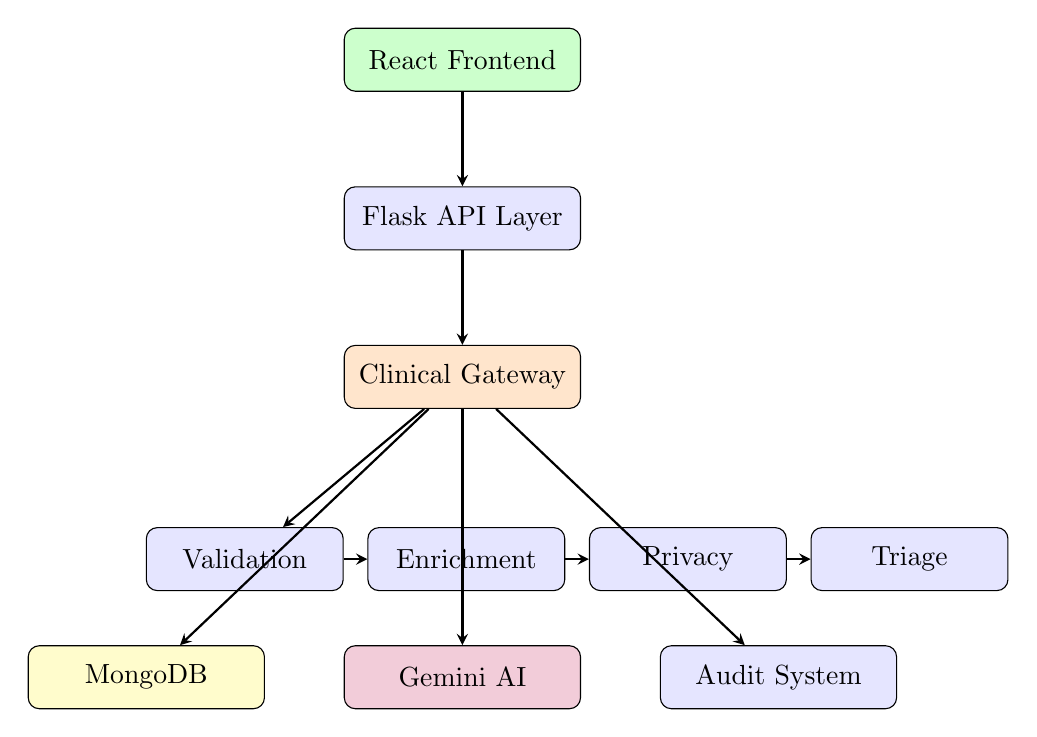
\begin{tikzpicture}[
    node distance=1.2cm,
    box/.style={rectangle, draw, rounded corners, minimum width=3cm, minimum height=0.8cm, align=center, fill=blue!10},
    arrow/.style={->, >=stealth, thick}
]
    % Frontend
    \node[box, fill=green!20] (frontend) {React Frontend};
    
    % API Gateway
    \node[box, below=of frontend] (api) {Flask API Layer};
    
    % Gateway
    \node[box, below=of api, fill=orange!20] (gateway) {Clinical Gateway};
    
    % Handlers
    \node[box, below left=1.5cm and 0cm of gateway, minimum width=2.5cm] (valid) {Validation};
    \node[box, right=0.3cm of valid, minimum width=2.5cm] (enrich) {Enrichment};
    \node[box, right=0.3cm of enrich, minimum width=2.5cm] (privacy) {Privacy};
    \node[box, right=0.3cm of privacy, minimum width=2.5cm] (triage) {Triage};
    
    % AI and DB
    \node[box, below=3cm of gateway, fill=purple!20] (ai) {Gemini AI};
    \node[box, left=1cm of ai, fill=yellow!20] (mongodb) {MongoDB};
    \node[box, right=1cm of ai] (audit) {Audit System};
    
    % Arrows
    \draw[arrow] (frontend) -- (api);
    \draw[arrow] (api) -- (gateway);
    \draw[arrow] (gateway) -- (valid);
    \draw[arrow] (valid) -- (enrich);
    \draw[arrow] (enrich) -- (privacy);
    \draw[arrow] (privacy) -- (triage);
    \draw[arrow] (gateway) -- (ai);
    \draw[arrow] (gateway) -- (mongodb);
    \draw[arrow] (gateway) -- (audit);
\end{tikzpicture}
\caption{EarlyCare Gateway System Architecture}
\end{figure}

\section{Data Flow Pipeline}

The clinical data processing follows a well-defined pipeline:

\begin{enumerate}[label=\textbf{Step \arabic*:}]
    \item \textbf{Ingestion}: The React frontend sends a Patient Record containing symptoms, vital signs, and attachments via HTTP POST request.
    
    \item \textbf{Gateway Entry}: The request enters the \texttt{ClinicalGateway} through the Flask API layer, where initial request parsing occurs.
    
    \item \textbf{Processing Chain}: The request passes through a chain of specialized handlers:
    \begin{itemize}
        \item \texttt{ValidationHandler}: Verifies data integrity, including valid Fiscal Codes and realistic vital sign ranges.
        \item \texttt{EnrichmentHandler}: Adds calculated metadata such as patient age from date of birth and BMI calculations.
        \item \texttt{PrivacyHandler}: Anonymizes sensitive fields before external AI processing.
        \item \texttt{TriageHandler}: Calculates initial urgency scores based on configured clinical rules.
    \end{itemize}
    
    \item \textbf{Strategy Execution}: The system selects the appropriate AI strategy (e.g., \texttt{GeminiStrategy}) to analyze the clinical data.
    
    \item \textbf{Observer Notification}: Auditing and Metrics systems record the transaction results for compliance and analytics.
    
    \item \textbf{Persistence}: Validated and enriched data is stored in MongoDB collections.
    
    \item \textbf{Response}: The complete, analyzed result is returned to the Frontend for display.
\end{enumerate}

\section{Component Interaction}

\subsection{Frontend-Backend Communication}

The frontend communicates with the backend through a RESTful API interface. All requests include credentials for session management:

\begin{lstlisting}[language=JavaScript, caption=Frontend API Call Example]
const response = await fetch(getApiUrl('/api/patient/search'), {
    method: 'POST',
    headers: { 'Content-Type': 'application/json' },
    credentials: 'include',
    body: JSON.stringify({ fiscal_code: searchCode })
});
\end{lstlisting}

\subsection{CORS Configuration}

Cross-Origin Resource Sharing is configured to allow the frontend application to communicate with the backend API:

\begin{lstlisting}[language=Python, caption=CORS Configuration]
CORS(app, 
     resources={
         r"/api/*": {
             "origins": allowed_origins,
             "methods": ["GET", "POST", "PUT", "DELETE", "OPTIONS"],
             "allow_headers": ["Content-Type", "Authorization"],
             "supports_credentials": True
         }
     })
\end{lstlisting}

\newpage

%==========================================
% CHAPTER 3: DESIGN PATTERNS
%==========================================
\chapter{Design Patterns Analysis}

This chapter provides an in-depth analysis of the Gang of Four (GoF) design patterns and their application within the EarlyCare Gateway system. We examine both the patterns that are currently implemented in the codebase and those that represent architectural opportunities for future development.

\section{Understanding Design Patterns}

Design patterns are reusable solutions to common software design problems. They represent best practices evolved over time by experienced software developers. The Gang of Four (GoF) patterns, documented by Erich Gamma, Richard Helm, Ralph Johnson, and John Vlissides, are categorized into three types:

\begin{itemize}
    \item \textbf{Creational Patterns}: Deal with object creation mechanisms
    \item \textbf{Structural Patterns}: Concern class and object composition
    \item \textbf{Behavioral Patterns}: Focus on communication between objects
\end{itemize}

\section{Strategy Pattern}

\subsection{Pattern Definition}
The \textbf{Strategy Pattern} is a behavioral design pattern that enables selecting an algorithm at runtime. Instead of implementing a single algorithm directly, code receives run-time instructions as to which in a family of algorithms to use. This pattern defines a family of algorithms, encapsulates each one, and makes them interchangeable.

\subsection{Implementation Status: PARTIALLY IMPLEMENTED}

The Strategy pattern is \textbf{partially implemented} in the AI diagnostics module. The current architecture provides the foundation for strategy-based AI model selection:

\begin{lstlisting}[language=Python, caption=Current AI Implementation (medical\_diagnostics.py)]
class MedicalDiagnosticsAI:
    def __init__(self, api_key: str):
        self.api_key = api_key
        genai.configure(api_key=api_key)
        self.model = genai.GenerativeModel('gemini-3-flash-preview')
        self.model_name = 'gemini-3-flash-preview'
    
    def generate_diagnosis(self, patient_data: Dict) -> Dict:
        max_retries = 3
        for attempt in range(max_retries):
            try:
                return self._generate_with_gemini(patient_data)
            except Exception as e:
                # Retry logic with exponential backoff
                wait_time = retry_delay * (2 ** attempt)
                time.sleep(wait_time)
\end{lstlisting}

\subsection{Current Implementation Analysis}
The system currently uses Google Gemini as its AI engine. While not a full Strategy pattern implementation, the architecture is \textbf{strategy-ready}:
\begin{itemize}
    \item The \texttt{MedicalDiagnosticsAI} class encapsulates the AI algorithm
    \item The \texttt{\_generate\_with\_gemini()} method is the concrete strategy
    \item Configuration allows API key injection, enabling different provider instances
\end{itemize}

\subsection{Recommended Full Implementation}
To fully implement the Strategy pattern, the code should be refactored as:

\begin{lstlisting}[language=Python, caption=Proposed Strategy Pattern]
from abc import ABC, abstractmethod

class DiagnosticStrategy(ABC):
    @abstractmethod
    def generate_diagnosis(self, patient_data: Dict) -> Dict:
        pass

class GeminiStrategy(DiagnosticStrategy):
    def generate_diagnosis(self, patient_data: Dict) -> Dict:
        # Google Gemini implementation
        pass

class OpenAIStrategy(DiagnosticStrategy):
    def generate_diagnosis(self, patient_data: Dict) -> Dict:
        # OpenAI GPT implementation
        pass

class DiagnosticEngine:
    def __init__(self, strategy: DiagnosticStrategy):
        self._strategy = strategy
    
    def set_strategy(self, strategy: DiagnosticStrategy):
        self._strategy = strategy
    
    def analyze(self, patient_data: Dict) -> Dict:
        return self._strategy.generate_diagnosis(patient_data)
\end{lstlisting}

\subsection{Benefits of Full Implementation}
\begin{itemize}
    \item Hot-swapping AI models without code changes
    \item Specialty-specific strategies (Cardiology, Neurology, etc.)
    \item A/B testing between different AI providers
    \item Fallback mechanisms when one provider fails
\end{itemize}

\section{Chain of Responsibility Pattern}

\subsection{Pattern Definition}
The \textbf{Chain of Responsibility} is a behavioral pattern that allows passing requests along a chain of handlers. Upon receiving a request, each handler decides either to process the request or to pass it to the next handler in the chain.

\subsection{Implementation Status: CONCEPTUAL / NOT IMPLEMENTED}

The Chain of Responsibility pattern is \textbf{described in the architectural vision} but not explicitly implemented as a formal pattern in the current codebase. The conceptual handlers include:

\begin{itemize}
    \item \texttt{ValidationHandler}: Would validate data integrity
    \item \texttt{EnrichmentHandler}: Would add calculated metadata
    \item \texttt{PrivacyHandler}: Would anonymize sensitive data
    \item \texttt{TriageHandler}: Would calculate urgency scores
\end{itemize}

\subsection{Current Equivalent Implementation}
Instead of a formal handler chain, the current implementation uses:

\begin{enumerate}
    \item \textbf{Inline Validation}: Field validation within route handlers
    \item \textbf{Model Methods}: The \texttt{Patient.anonymize()} method for privacy
    \item \textbf{Calculated Properties}: \texttt{Patient.calculate\_age()} for enrichment
\end{enumerate}

\begin{lstlisting}[language=Python, caption=Current Validation Approach (app.py)]
@app.route('/api/patient/create', methods=['POST'])
@require_login
def create_patient():
    data = request.json
    
    # Inline validation (not a formal handler)
    required_fields = ['nome', 'cognome', 'data_nascita']
    for field in required_fields:
        if not data.get(field):
            return jsonify({'error': f'Missing: {field}'}), 400
    
    # Enrichment inline
    patient = Patient(...)
    patient.calculate_age()  # Enrichment method
    
    # No formal handler chain
    db.save_patient(patient)
\end{lstlisting}

\subsection{Recommended Implementation}
\begin{lstlisting}[language=Python, caption=Proposed Chain of Responsibility]
from abc import ABC, abstractmethod

class Handler(ABC):
    def __init__(self):
        self._next_handler = None
    
    def set_next(self, handler: 'Handler') -> 'Handler':
        self._next_handler = handler
        return handler
    
    @abstractmethod
    def handle(self, request: Dict) -> Dict:
        if self._next_handler:
            return self._next_handler.handle(request)
        return request

class ValidationHandler(Handler):
    def handle(self, request: Dict) -> Dict:
        # Validate required fields
        if not request.get('nome'):
            raise ValueError("Nome required")
        return super().handle(request)

class EnrichmentHandler(Handler):
    def handle(self, request: Dict) -> Dict:
        # Add calculated fields
        request['age'] = calculate_age(request['data_nascita'])
        return super().handle(request)

# Usage
chain = ValidationHandler()
chain.set_next(EnrichmentHandler()).set_next(PrivacyHandler())
result = chain.handle(patient_data)
\end{lstlisting}

\section{Observer Pattern}

\subsection{Pattern Definition}
The \textbf{Observer Pattern} is a behavioral pattern where an object (subject) maintains a list of its dependents (observers) and notifies them automatically of any state changes. This is useful for implementing distributed event handling systems.

\subsection{Implementation Status: NOT IMPLEMENTED}

The Observer pattern is \textbf{referenced in documentation} but \textbf{not implemented} in the current codebase. A comment in \texttt{app.py} indicates:

\begin{lstlisting}[language=Python, caption=Evidence from app.py line 1086]
# Metrics observer removed
\end{lstlisting}

\subsection{Conceptual Design}
The architectural vision describes:
\begin{itemize}
    \item \texttt{AuditObserver}: Would log system actions
    \item \texttt{MetricsObserver}: Would track performance metrics
\end{itemize}

\subsection{Current Logging Approach}
Instead of observers, the system uses direct logging:

\begin{lstlisting}[language=Python, caption=Current Logging (mongodb\_repository.py)]
import logging
logger = logging.getLogger(__name__)

def save_patient(self, patient: Patient) -> bool:
    try:
        self.patients_collection.insert_one(patient_dict)
        logger.info(f"Saved patient: {patient.patient_id}")
        return True
    except Exception as e:
        logger.error(f"Error saving patient: {e}")
        return False
\end{lstlisting}

\subsection{Recommended Implementation}
\begin{lstlisting}[language=Python, caption=Proposed Observer Pattern]
from abc import ABC, abstractmethod
from typing import List

class Observer(ABC):
    @abstractmethod
    def update(self, event: str, data: Dict):
        pass

class AuditObserver(Observer):
    def update(self, event: str, data: Dict):
        audit_log = {
            'event': event,
            'timestamp': datetime.now(),
            'data': data,
            'actor': data.get('doctor_id')
        }
        db.audit_logs.insert_one(audit_log)

class MetricsObserver(Observer):
    def update(self, event: str, data: Dict):
        # Track metrics for analytics
        metrics.increment(event)

class ClinicalGateway:
    def __init__(self):
        self._observers: List[Observer] = []
    
    def attach(self, observer: Observer):
        self._observers.append(observer)
    
    def notify(self, event: str, data: Dict):
        for observer in self._observers:
            observer.update(event, data)
    
    def process_patient(self, patient_data):
        # Process patient
        result = self._process(patient_data)
        # Notify all observers
        self.notify('patient_created', {'patient_id': result.id})
        return result
\end{lstlisting}

\section{Facade Pattern}

\subsection{Pattern Definition}
The \textbf{Facade Pattern} is a structural pattern that provides a simplified interface to a complex subsystem. It doesn't encapsulate the subsystem but provides a unified interface that makes the subsystem easier to use.

\subsection{Implementation Status: NOT IMPLEMENTED}

The Facade pattern is \textbf{mentioned for future HL7/FHIR integration} but no \texttt{src/facade} directory or facade classes exist in the current codebase.

\subsection{Architectural Vision}
The README references: \textit{"Facade Pattern: (In src/facade) Used to standardize interactions with external clinical systems (like potential future HL7/FHIR integrations)"}

\subsection{Recommended Implementation for Healthcare Interoperability}
\begin{lstlisting}[language=Python, caption=Proposed Facade for Clinical Systems]
class ClinicalSystemsFacade:
    """Simplified interface for external clinical systems"""
    
    def __init__(self):
        self._hl7_client = HL7Client()
        self._fhir_client = FHIRClient()
        self._dicom_client = DICOMClient()
    
    def send_patient_to_ehr(self, patient: Patient):
        """Send patient to external EHR system"""
        fhir_patient = self._convert_to_fhir(patient)
        return self._fhir_client.create_patient(fhir_patient)
    
    def receive_lab_results(self, patient_id: str):
        """Receive lab results from external LIS"""
        hl7_message = self._hl7_client.query_results(patient_id)
        return self._parse_hl7_results(hl7_message)
    
    def fetch_imaging(self, study_id: str):
        """Fetch medical images from PACS"""
        return self._dicom_client.retrieve_study(study_id)
\end{lstlisting}

\section{Decorator Pattern}

\subsection{Pattern Definition}
The \textbf{Decorator Pattern} is a structural pattern that allows adding new behaviors to objects dynamically by placing them inside wrapper objects.

\subsection{Implementation Status: IMPLEMENTED}

The Decorator pattern is \textbf{fully implemented} using Python decorators for cross-cutting concerns like authentication:

\begin{lstlisting}[language=Python, caption=Authentication Decorator (app.py)]
from functools import wraps

def require_login(f):
    """Decorator to require doctor login for protected routes"""
    @wraps(f)
    def decorated_function(*args, **kwargs):
        if 'doctor_id' not in session:
            return jsonify({'error': 'Non autorizzato'}), 401
        return f(*args, **kwargs)
    return decorated_function

# Usage on protected routes
@app.route('/api/patient/search', methods=['POST'])
@require_login
def search_patient():
    # Only accessible by authenticated doctors
    ...
\end{lstlisting}

\subsection{Benefits in Current Implementation}
\begin{itemize}
    \item Separates authentication logic from business logic
    \item Easily applied to any route requiring protection
    \item Follows DRY (Don't Repeat Yourself) principle
    \item Can be stacked with other decorators
\end{itemize}

\section{Pattern Implementation Summary}

\begin{table}[h]
\centering
\begin{tabular}{llp{6cm}}
\toprule
\textbf{Pattern} & \textbf{Status} & \textbf{Notes} \\
\midrule
Strategy & Partial & AI module is strategy-ready but uses single implementation \\
Chain of Responsibility & Conceptual & Described in architecture, implemented inline \\
Observer & Not Implemented & Referenced but removed from codebase \\
Facade & Not Implemented & Planned for future HL7/FHIR integration \\
Decorator & Implemented & Used for authentication (\texttt{@require\_login}) \\
\bottomrule
\end{tabular}
\caption{Design Pattern Implementation Status}
\end{table}

\section{Recommendations}

Based on the analysis, the following pattern implementations are recommended for future development:

\begin{enumerate}
    \item \textbf{Priority 1 - Strategy Pattern}: Formalize the AI strategy to enable multiple providers
    \item \textbf{Priority 2 - Observer Pattern}: Implement for comprehensive audit logging
    \item \textbf{Priority 3 - Chain of Responsibility}: Create formal validation pipeline
    \item \textbf{Priority 4 - Facade Pattern}: Develop when implementing HL7/FHIR
\end{enumerate}

\newpage

%==========================================
% CHAPTER 4: TECHNOLOGY STACK
%==========================================
\chapter{Technology Stack}

EarlyCare Gateway utilizes a modern, well-integrated technology stack designed for reliability, scalability, and maintainability.

\section{Backend Technologies}

\subsection{Python Flask Framework}
The backend is built using Flask, a lightweight micro-framework that provides flexibility without imposing unnecessary constraints.

\begin{table}[h]
\centering
\begin{tabular}{ll}
\toprule
\textbf{Component} & \textbf{Version/Details} \\
\midrule
Python & 3.8+ \\
Flask & 3.0.0+ \\
Flask-CORS & 4.0.0+ \\
\bottomrule
\end{tabular}
\caption{Core Backend Framework}
\end{table}

\subsection{AI Integration}
\begin{itemize}
    \item \textbf{Google Generative AI SDK}: \texttt{google-generativeai >= 0.3.0}
    \item Model: \texttt{gemini-3-flash-preview}
    \item Supports multimodal input (text + images)
\end{itemize}

\subsection{Data Processing Libraries}
\begin{itemize}
    \item \textbf{NumPy}: Numerical computing
    \item \textbf{Pandas}: Data manipulation and analysis
    \item \textbf{PIL (Pillow)}: Image processing for medical attachments
    \item \textbf{PyPDF2}: PDF parsing and generation
    \item \textbf{ReportLab}: Professional PDF report generation
\end{itemize}

\subsection{Database Connectivity}
\begin{itemize}
    \item \textbf{PyMongo}: MongoDB driver for Python (>= 4.6.0)
    \item SSL/TLS support for secure connections
    \item Connection pooling for performance
\end{itemize}

\section{Frontend Technologies}

\subsection{React 18 with Vite}
The frontend leverages modern React development practices:

\begin{table}[h]
\centering
\begin{tabular}{ll}
\toprule
\textbf{Technology} & \textbf{Version/Details} \\
\midrule
React & 18.2.0+ \\
React DOM & 18.2.0+ \\
Vite & 5.0.8+ \\
@vitejs/plugin-react & 4.2.1+ \\
\bottomrule
\end{tabular}
\caption{Frontend Framework Stack}
\end{table}

\subsection{State Management}
\begin{itemize}
    \item React Hooks (useState, useEffect)
    \item Context API for global state
    \item SessionStorage for data persistence
\end{itemize}

\subsection{Styling}
\begin{itemize}
    \item Modern vanilla CSS with Glassmorphism design language
    \item Responsive layout optimized for dark/light mode
    \item CSS custom properties for theming
\end{itemize}

\section{Infrastructure}

\subsection{Database}
\begin{itemize}
    \item \textbf{MongoDB}: NoSQL database for flexible schema management
    \item MongoDB Atlas for cloud deployment
    \item Polymorphic clinical data storage
\end{itemize}

\subsection{Containerization}
\begin{itemize}
    \item \textbf{Docker}: Container runtime
    \item \textbf{Docker Compose}: Multi-container orchestration
    \item Nginx for frontend static file serving
\end{itemize}

\subsection{Dependencies Summary}

\begin{lstlisting}[caption=Key Backend Dependencies]
# Core
flask>=3.0.0
flask-cors>=4.0.0
pymongo>=4.6.0
google-generativeai>=0.3.0

# Data Processing
numpy>=1.21.0
pandas>=1.3.0

# PDF Generation
reportlab>=4.0.0
PyPDF2>=3.0.0

# Security
cryptography>=41.0.0

# Italian Fiscal Code
codicefiscale>=0.9
\end{lstlisting}

\newpage

%==========================================
% CHAPTER 5: CORE COMPONENTS
%==========================================
\chapter{Core Components}

\section{Patient Management Module}

\subsection{Patient Model}
The Patient model represents comprehensive patient demographic and clinical information:

\begin{lstlisting}[language=Python, caption=Patient Model Structure]
@dataclass
class Patient:
    # Required fields
    patient_id: str
    nome: str
    cognome: str
    data_nascita: datetime
    comune_nascita: str
    codice_fiscale: str
    
    # Optional fields
    data_decesso: Optional[datetime] = None
    allergie: List[str] = field(default_factory=list)
    malattie_permanenti: List[str] = field(default_factory=list)
    gender: Optional[Gender] = None
    age: Optional[int] = None
    is_foreign: bool = False
\end{lstlisting}

\subsection{Dual Identity System}
The system supports two patient identification approaches:

\begin{enumerate}
    \item \textbf{Italian Citizens}: Validated via strict Fiscal Code algorithms with OMOCODA support
    \item \textbf{Foreign Citizens}: Automatic generation of unique internal IDs (format: \texttt{XX-YYYY})
\end{enumerate}

\subsection{Fiscal Code Calculation}
The system includes a complete Italian Fiscal Code calculator:

\begin{lstlisting}[language=Python, caption=Fiscal Code Generation]
def calculate_codice_fiscale(
    nome: str,
    cognome: str,
    data_nascita,
    comune_nascita: str,
    sesso: str
) -> Optional[str]:
    # Uses codicefiscale library with cadastral code lookup
    municipality_code = get_municipality_code(comune_nascita)
    return build(surname=cognome, name=nome, ...)
\end{lstlisting}

\section{Doctor Authentication Module}

\subsection{Doctor Model}
Doctors are authenticated users who can manage patients and clinical records:

\begin{lstlisting}[language=Python, caption=Doctor Model]
@dataclass
class Doctor:
    doctor_id: str  # Unique mnemonic ID (e.g., MR7X9Z)
    nome: str
    cognome: str
    specializzazione: str
    ospedale_affiliato: str
    password_hash: str
    created_at: datetime
    is_active: bool = True
\end{lstlisting}

\subsection{Unique ID Generation}
Doctor IDs are generated using a secure random algorithm:

\begin{lstlisting}[language=Python, caption=Doctor ID Generation]
@staticmethod
def generate_doctor_id(nome: str, cognome: str) -> str:
    # Format: FirstLetterLastLetterRandomChars (6 chars)
    first_letter_nome = nome[0].upper()
    first_letter_cognome = cognome[0].upper()
    chars = string.ascii_uppercase + string.digits
    random_suffix = ''.join(secrets.choice(chars) for _ in range(4))
    return f"{first_letter_nome}{first_letter_cognome}{random_suffix}"
\end{lstlisting}

\section{Clinical Records Module}

\subsection{Record Structure}
Clinical records capture comprehensive visit information:

\begin{itemize}
    \item \textbf{Encounter Information}: ID, timestamp, priority level
    \item \textbf{Chief Complaint}: Primary reason for visit
    \item \textbf{Symptoms}: Detailed symptom description
    \item \textbf{Vital Signs}: Blood pressure, heart rate, temperature, oxygen saturation
    \item \textbf{Attachments}: Medical images and documents
    \item \textbf{Notes}: Clinical observations
\end{itemize}

\subsection{Vital Signs Tracking}
The system tracks and validates critical vital signs:

\begin{table}[h]
\centering
\begin{tabular}{lll}
\toprule
\textbf{Vital Sign} & \textbf{Unit} & \textbf{Normal Range} \\
\midrule
Blood Pressure & mmHg & 90/60 - 120/80 \\
Heart Rate & bpm & 60 - 100 \\
Temperature & °C & 36.1 - 37.2 \\
Oxygen Saturation & \% & 95 - 100 \\
Respiratory Rate & breaths/min & 12 - 20 \\
\bottomrule
\end{tabular}
\caption{Vital Signs Reference Ranges}
\end{table}

\section{PDF Export Module}

The system generates professional clinical reports using ReportLab:

\begin{itemize}
    \item Complete patient demographics
    \item All clinical records with vital signs
    \item Attached images embedded in PDF
    \item AI-generated diagnoses (when available)
    \item Smart pagination for clean document flow
\end{itemize}

\newpage

%==========================================
% CHAPTER 6: AI AND DIAGNOSTICS ENGINE
%==========================================
\chapter{AI and Diagnostics Engine}

\section{Overview}

The AI module in EarlyCare Gateway is not a simple chatbot—it is a \textbf{Structured Clinical Analyst} designed to provide comprehensive diagnostic support to healthcare professionals.

\section{Multimodal Analysis Capabilities}

\subsection{Input Processing}
The AI engine accepts multiple data types simultaneously:

\begin{enumerate}
    \item \textbf{Structured Clinical Data}: JSON-formatted patient information including:
    \begin{itemize}
        \item Patient demographics
        \item Medical history
        \item Current symptoms
        \item Vital signs
        \item Current medications
    \end{itemize}
    
    \item \textbf{Medical Images}: Base64-encoded images including:
    \begin{itemize}
        \item X-ray images
        \item ECG tracings
        \item Skin photographs
        \item Other diagnostic images
    \end{itemize}
\end{enumerate}

\subsection{Image Processing Pipeline}
\begin{lstlisting}[language=Python, caption=Image Processing for AI]
for att in attachments:
    if att['type'].startswith('image/'):
        # Decode base64 image
        image_data = base64.b64decode(att['content'])
        image = Image.open(io.BytesIO(image_data))
        
        # Convert to RGB for Gemini compatibility
        if image.mode != 'RGB':
            image = image.convert('RGB')
        
        image_parts.append({'name': file_name, 'image': image})
\end{lstlisting}

\section{Structured Output Format}

The AI is configured through careful prompt engineering to return structured clinical assessments:

\begin{enumerate}
    \item \textbf{Clinical Data Analysis}: Evaluation of symptom consistency and medical history relevance
    
    \item \textbf{Image Interpretation}: Detailed analysis of any attached medical images
    
    \item \textbf{Presumptive Diagnosis}: Primary diagnosis ranked by probability with clinical reasoning
    
    \item \textbf{Differential Diagnoses}: Alternative diagnoses with supporting and contradicting evidence
    
    \item \textbf{Recommended Tests}: Suggested diagnostic examinations with expected outcomes
    
    \item \textbf{Treatment Plan}: Medication recommendations with dosages and non-pharmacological interventions
    
    \item \textbf{Monitoring Plan}: Parameters to track and follow-up schedule
    
    \item \textbf{Urgency Assessment}: Priority level and intervention timeline
\end{enumerate}

\section{Retry Logic and Error Handling}

The system implements robust error handling with exponential backoff:

\begin{lstlisting}[language=Python, caption=Retry Logic Implementation]
def generate_diagnosis(self, patient_data: Dict) -> Dict:
    max_retries = 3
    retry_delay = 1  # seconds
    
    for attempt in range(max_retries):
        try:
            return self._generate_with_gemini(patient_data)
        except Exception as e:
            if attempt == max_retries - 1:
                raise
            wait_time = retry_delay * (2 ** attempt)
            time.sleep(wait_time)
\end{lstlisting}

\section{Medical Chatbot}

A separate AI instance powers the medical chatbot feature:

\begin{itemize}
    \item Dedicated API key for isolation
    \item Conversational interface for medical queries
    \item Strict medical-only response policy
    \item Real-time response generation
\end{itemize}

\section{AI Configuration}

\begin{lstlisting}[language=Python, caption=AI Generation Configuration]
response = self.model.generate_content(
    content_parts,
    generation_config=genai.types.GenerationConfig(
        temperature=0.3,      # Low temperature for consistency
        top_p=0.95,
        top_k=40,
        max_output_tokens=16384,
        candidate_count=1,
    )
)
\end{lstlisting}

\newpage

%==========================================
% CHAPTER 7: SECURITY AND PRIVACY
%==========================================
\chapter{Security and Privacy}

\section{Authentication System}

\subsection{Doctor Registration}
The registration process includes:
\begin{itemize}
    \item Unique mnemonic Doctor ID generation
    \item Password strength validation (minimum 6 characters)
    \item SHA-256 password hashing
    \item Duplicate ID prevention
\end{itemize}

\subsection{Session Management}
\begin{lstlisting}[language=Python, caption=Session Configuration]
app.config['SESSION_COOKIE_SECURE'] = is_production  # HTTPS only
app.config['SESSION_COOKIE_HTTPONLY'] = True
app.config['SESSION_COOKIE_SAMESITE'] = 'None' if is_production else 'Lax'
app.config['PERMANENT_SESSION_LIFETIME'] = 86400 * 7  # 7 days
\end{lstlisting}

\subsection{Password Security}
\begin{lstlisting}[language=Python, caption=Password Hashing]
@staticmethod
def hash_password(password: str) -> str:
    """Hash a password using SHA-256"""
    return hashlib.sha256(password.encode()).hexdigest()

@staticmethod
def verify_password(password: str, password_hash: str) -> bool:
    """Verify a password against its hash"""
    return Doctor.hash_password(password) == password_hash
\end{lstlisting}

\section{Data Protection}

\subsection{Data at Rest}
\begin{itemize}
    \item MongoDB data structured to separate PII from clinical data
    \item Encrypted storage options through MongoDB Atlas
    \item Secure database access credentials management
\end{itemize}

\subsection{Data in Transit}
\begin{itemize}
    \item Forced HTTPS on production deployments
    \item TLS/SSL encryption for database connections
    \item Secure cookie transmission
\end{itemize}

\subsection{Data Anonymization}
The system provides anonymization capabilities for external processing:

\begin{lstlisting}[language=Python, caption=Patient Anonymization]
def anonymize(self) -> 'Patient':
    """Create anonymized patient record."""
    return Patient(
        patient_id="ANONYMIZED",
        nome="ANONYMIZED",
        cognome="ANONYMIZED",
        data_nascita=datetime(self.data_nascita.year, 1, 1),
        comune_nascita="ANONYMIZED",
        codice_fiscale="ANONYMIZED",
        allergie=self.allergie.copy(),
        malattie_permanenti=self.malattie_permanenti.copy()
    )
\end{lstlisting}

\section{Audit Logging}

Every significant action is logged for accountability:

\begin{itemize}
    \item Patient record creation and modification
    \item Clinical record access
    \item Export operations
    \item Authentication events (login, logout, registration)
    \item AI diagnostic requests
\end{itemize}

\section{Compliance Considerations}

The system is designed with compliance in mind:

\begin{itemize}
    \item \textbf{HIPAA}: Health Insurance Portability and Accountability Act guidelines
    \item \textbf{GDPR}: General Data Protection Regulation requirements
    \item Audit trail maintenance
    \item Data minimization principles
    \item User consent management capabilities
\end{itemize}

\newpage

%==========================================
% CHAPTER 8: DATABASE ARCHITECTURE
%==========================================
\chapter{Database Architecture}

\section{MongoDB Collections}

The MongoDB database uses five primary collections:

\subsection{Users Collection (doctors)}
Stores doctor credentials and profiles:

\begin{lstlisting}[caption=Doctors Collection Schema]
{
    "_id": ObjectId,
    "doctor_id": String (indexed, unique),
    "nome": String,
    "cognome": String,
    "specializzazione": String,
    "ospedale_affiliato": String,
    "password_hash": String,
    "created_at": Date,
    "last_login": Date,
    "is_active": Boolean
}
\end{lstlisting}

\subsection{Patients Collection}
Stores patient demographics:

\begin{lstlisting}[caption=Patients Collection Schema]
{
    "_id": ObjectId,
    "patient_id": String (indexed),
    "nome": String (required),
    "cognome": String (required),
    "data_nascita": Date (required),
    "comune_nascita": String (required),
    "codice_fiscale": String (required, indexed),
    "allergie": Array[String],
    "malattie_permanenti": Array[String],
    "gender": Enum["male", "female", "other", "unknown"],
    "is_foreign": Boolean,
    "created_at": Date,
    "updated_at": Date
}
\end{lstlisting}

\subsection{Clinical Records Collection}
Links patients to encounters:

\begin{lstlisting}[caption=Clinical Records Schema]
{
    "_id": ObjectId,
    "encounter_id": String (indexed, unique),
    "patient_id": String (indexed),
    "chief_complaint": String,
    "symptoms": String,
    "priority": Enum["routine", "urgent", "emergency"],
    "vital_signs": {
        "blood_pressure": String,
        "heart_rate": String,
        "temperature": String,
        "oxygen_saturation": String,
        "respiratory_rate": String
    },
    "attachments": Array[Object],
    "notes": String,
    "timestamp": Date,
    "doctor_id": String
}
\end{lstlisting}

\subsection{Audit Logs Collection}
Immutable history of system actions:

\begin{lstlisting}[caption=Audit Logs Schema]
{
    "_id": ObjectId,
    "action": String,
    "actor_id": String,
    "target_type": String,
    "target_id": String,
    "timestamp": Date,
    "details": Object
}
\end{lstlisting}

\section{Indexing Strategy}

Strategic indexes are created for optimal query performance:

\begin{table}[h]
\centering
\begin{tabular}{lll}
\toprule
\textbf{Collection} & \textbf{Field(s)} & \textbf{Type} \\
\midrule
patients & codice\_fiscale & Unique \\
patients & patient\_id & Unique \\
patient\_records & encounter\_id & Unique \\
patient\_records & patient\_id & Regular \\
doctors & doctor\_id & Unique \\
audit\_logs & timestamp & Regular \\
\bottomrule
\end{tabular}
\caption{Database Indexes}
\end{table}

\section{Connection Configuration}

\begin{lstlisting}[language=Python, caption=MongoDB Connection]
connection_params = {
    'serverSelectionTimeoutMS': 10000,
    'connectTimeoutMS': 20000,
    'socketTimeoutMS': 20000,
    'tls': True,
    'tlsAllowInvalidCertificates': True
}

self.client = MongoClient(connection_string, **connection_params)
\end{lstlisting}

\newpage

%==========================================
% CHAPTER 9: DEPLOYMENT GUIDE
%==========================================
\chapter{Deployment Guide}

\section{Docker Deployment (Recommended)}

\subsection{Prerequisites}
\begin{itemize}
    \item Docker Engine installed
    \item Docker Compose installed
    \item Environment variables configured
\end{itemize}

\subsection{Quick Start}
\begin{lstlisting}[language=bash, caption=Docker Deployment]
# Clone the repository
git clone https://github.com/your-repo/earlycare-gateway.git
cd earlycare-gateway

# Configure environment variables
cp .env.example .env
# Edit .env with your credentials

# Start the full stack
docker-compose up -d --build
\end{lstlisting}

\subsection{Docker Compose Configuration}
\begin{lstlisting}[caption=Docker Compose Services]
services:
  backend:
    build:
      context: .
      dockerfile: Dockerfile
    ports:
      - "5000:5000"
    environment:
      - MONGODB_CONNECTION_STRING=${MONGODB_CONNECTION_STRING}
      - GEMINI_API_KEY=${GEMINI_API_KEY}
      - FLASK_SECRET_KEY=${FLASK_SECRET_KEY}
    
  frontend:
    build:
      context: ./frontend
      dockerfile: Dockerfile
    ports:
      - "80:80"
    depends_on:
      - backend
\end{lstlisting}

\section{Manual Deployment}

\subsection{Backend Setup}
\begin{lstlisting}[language=bash, caption=Backend Manual Setup]
cd backend
python -m venv venv

# Windows
venv\Scripts\activate

# Linux/Mac
source venv/bin/activate

pip install -r requirements.txt

# Create .env file
echo "GEMINI_API_KEY=your_key" > .env
echo "MONGODB_CONNECTION_STRING=your_connection" >> .env

# Start the server
python webapp/app.py
\end{lstlisting}

\subsection{Frontend Setup}
\begin{lstlisting}[language=bash, caption=Frontend Manual Setup]
cd frontend
npm install
npm run dev
\end{lstlisting}

\section{Environment Variables}

\begin{table}[h]
\centering
\begin{tabular}{lp{8cm}}
\toprule
\textbf{Variable} & \textbf{Description} \\
\midrule
GEMINI\_API\_KEY & Google Gemini API key for AI diagnostics \\
CHATBOT\_GEMINI\_API\_KEY & Separate API key for chatbot \\
MONGODB\_CONNECTION\_STRING & MongoDB Atlas connection string \\
FLASK\_SECRET\_KEY & Secret key for session encryption \\
FRONTEND\_URL & Frontend URL for CORS configuration \\
VITE\_API\_URL & Backend API URL for frontend \\
\bottomrule
\end{tabular}
\caption{Required Environment Variables}
\end{table}

\section{Production Deployment (Render)}

The application is configured for deployment on Render.com:

\begin{enumerate}
    \item Create a new Web Service
    \item Connect GitHub repository
    \item Configure environment variables
    \item Set build command: \texttt{pip install -r requirements.txt}
    \item Set start command: \texttt{python webapp/app.py}
\end{enumerate}

\section{Troubleshooting}

\subsection{Common Issues}

\begin{itemize}
    \item \textbf{CORS Errors}: Check protocol (HTTP/HTTPS) and trailing slashes in URLs
    \item \textbf{AI Errors}: Ensure images are under 4MB and in standard formats
    \item \textbf{Database Connection}: Verify IP whitelist on MongoDB Atlas
    \item \textbf{Session Issues}: Verify cookie configuration for cross-domain scenarios
\end{itemize}

\newpage

%==========================================
% CHAPTER 10: FUTURE IMPROVEMENTS
%==========================================
\chapter{Future Improvements}

This chapter outlines planned enhancements and areas for improvement in the EarlyCare Gateway platform.

\section{Enhanced Security System}

\subsection{Current Limitations}
The current security implementation, while functional, has areas that could be strengthened:
\begin{itemize}
    \item SHA-256 password hashing (no salting)
    \item Session-based authentication only
    \item Basic role-based access control
\end{itemize}

\subsection{Proposed Improvements}

\subsubsection{Advanced Password Hashing}
Implement industry-standard password hashing algorithms:
\begin{itemize}
    \item \textbf{bcrypt}: Adaptive hashing with automatic salting
    \item \textbf{Argon2}: Memory-hard hashing for enhanced security
    \item Password complexity requirements enforcement
    \item Password history to prevent reuse
\end{itemize}

\subsubsection{Multi-Factor Authentication (MFA)}
\begin{itemize}
    \item TOTP (Time-based One-Time Password) support
    \item SMS/Email verification codes
    \item Hardware security key support (FIDO2/WebAuthn)
    \item Biometric authentication integration
\end{itemize}

\subsubsection{JWT-Based Authentication}
\begin{itemize}
    \item Stateless authentication for better scalability
    \item Refresh token rotation
    \item Token revocation mechanisms
    \item Fine-grained permission scopes
\end{itemize}

\subsubsection{Role-Based Access Control (RBAC)}
\begin{itemize}
    \item Hierarchical role definitions (Admin, Doctor, Nurse, Receptionist)
    \item Granular permissions per resource type
    \item Department-based access restrictions
    \item Audit logging for all access attempts
\end{itemize}

\section{Native Application Development}

\subsection{Motivation}
Converting the web application to a native desktop/mobile application offers several advantages:
\begin{itemize}
    \item Offline functionality for areas with limited connectivity
    \item Better system integration (notifications, file system access)
    \item Enhanced performance for data-intensive operations
    \item Improved security through local data encryption
\end{itemize}

\subsection{Proposed Technologies}

\subsubsection{Desktop Application}
\begin{itemize}
    \item \textbf{Electron}: Cross-platform desktop framework using web technologies
    \item \textbf{Tauri}: Lightweight alternative with Rust backend
    \item \textbf{Flutter Desktop}: Single codebase for all platforms
\end{itemize}

\subsubsection{Mobile Application}
\begin{itemize}
    \item \textbf{React Native}: Leverage existing React knowledge
    \item \textbf{Flutter}: High-performance cross-platform development
    \item Native development for iOS (Swift) and Android (Kotlin)
\end{itemize}

\subsubsection{Progressive Web App (PWA)}
As an intermediate step:
\begin{itemize}
    \item Service Workers for offline functionality
    \item Push notifications
    \item Home screen installation
    \item Background sync for data updates
\end{itemize}

\section{OCR for Attachment Recognition}

\subsection{Use Case}
Many clinical documents are scanned or photographed, making text extraction crucial for comprehensive analysis.

\subsection{Proposed Implementation}

\subsubsection{OCR Technologies}
\begin{itemize}
    \item \textbf{Tesseract OCR}: Open-source OCR engine
    \item \textbf{Google Cloud Vision API}: High-accuracy cloud-based OCR
    \item \textbf{Azure Computer Vision}: Microsoft's OCR service
    \item \textbf{Amazon Textract}: Document analysis service
\end{itemize}

\subsubsection{Document Types to Support}
\begin{itemize}
    \item Prescription documents
    \item Laboratory test results
    \item Referral letters
    \item Previous medical records
    \item Insurance documents
    \item Consent forms
\end{itemize}

\subsubsection{Integration Architecture}
\begin{lstlisting}[language=Python, caption=Proposed OCR Integration]
class DocumentProcessor:
    def process_attachment(self, attachment):
        if attachment.type == 'application/pdf':
            text = self.extract_pdf_text(attachment)
        elif attachment.type.startswith('image/'):
            text = self.perform_ocr(attachment)
        
        # Structure extracted data
        structured_data = self.parse_medical_document(text)
        return structured_data
    
    def perform_ocr(self, image):
        # Use Tesseract or cloud OCR
        return pytesseract.image_to_string(image)
\end{lstlisting}

\section{Additional Improvements}

\subsection{HL7 FHIR Integration}
\begin{itemize}
    \item Implement FHIR R4 resource models
    \item Enable interoperability with other healthcare systems
    \item Support for FHIR Questionnaire resources
    \item Bulk data export in FHIR format
\end{itemize}

\subsection{Advanced Analytics Dashboard}
\begin{itemize}
    \item Patient population statistics
    \item Disease trend analysis
    \item Doctor performance metrics
    \item AI diagnostic accuracy tracking
\end{itemize}

\subsection{Telemedicine Integration}
\begin{itemize}
    \item Video consultation capabilities
    \item Screen sharing for image review
    \item Secure messaging between providers
    \item Virtual waiting room functionality
\end{itemize}

\subsection{Enhanced AI Capabilities}
\begin{itemize}
    \item Multiple AI model support (OpenAI, Claude, Gemini)
    \item Specialty-specific diagnostic models
    \item Continuous learning from feedback
    \item Explainable AI for diagnosis transparency
\end{itemize}

\subsection{Appointment Scheduling}
\begin{itemize}
    \item Calendar integration
    \item Automated appointment reminders
    \item Patient self-scheduling portal
    \item Resource (room, equipment) management
\end{itemize}

\subsection{Prescription Management}
\begin{itemize}
    \item Electronic prescription generation
    \item Drug interaction checking
    \item Pharmacy integration
    \item Prescription history tracking
\end{itemize}

\subsection{Performance Optimizations}
\begin{itemize}
    \item Redis caching layer for frequently accessed data
    \item Database query optimization
    \item CDN integration for static assets
    \item Lazy loading for large data sets
\end{itemize}

\subsection{Accessibility Improvements}
\begin{itemize}
    \item WCAG 2.1 AA compliance
    \item Screen reader optimization
    \item Keyboard navigation enhancement
    \item High contrast mode support
\end{itemize}

\section{Implementation Roadmap}

\begin{table}[h]
\centering
\begin{tabular}{llc}
\toprule
\textbf{Phase} & \textbf{Feature} & \textbf{Priority} \\
\midrule
Phase 1 (Q1) & Enhanced Security (MFA, bcrypt) & High \\
Phase 1 (Q1) & OCR Integration & High \\
Phase 2 (Q2) & PWA Conversion & Medium \\
Phase 2 (Q2) & HL7 FHIR Support & Medium \\
Phase 3 (Q3) & Native Desktop App & Medium \\
Phase 3 (Q3) & Analytics Dashboard & Medium \\
Phase 4 (Q4) & Telemedicine Features & Low \\
Phase 4 (Q4) & Mobile Application & Low \\
\bottomrule
\end{tabular}
\caption{Implementation Roadmap}
\end{table}

\newpage

%==========================================
% CHAPTER 11: CONCLUSION
%==========================================
\chapter{Conclusion}

\section{Summary}

EarlyCare Gateway represents a significant advancement in clinical decision support systems, combining modern web technologies with state-of-the-art artificial intelligence to assist healthcare professionals in their daily practice.

Key achievements of this project include:

\begin{itemize}
    \item \textbf{Robust Architecture}: Implementation of a layered gateway architecture with well-defined design patterns ensuring maintainability and extensibility.
    
    \item \textbf{AI-Powered Diagnostics}: Integration of Google Gemini for multimodal analysis of clinical data and medical images, providing structured diagnostic support.
    
    \item \textbf{Comprehensive Patient Management}: Complete lifecycle management for patients with support for both Italian citizens and foreign patients.
    
    \item \textbf{Security-First Approach}: Implementation of authentication, authorization, and audit logging mechanisms designed with compliance in mind.
    
    \item \textbf{Modern Deployment}: Docker containerization for consistent deployment across environments.
\end{itemize}

\section{Technical Excellence}

The project demonstrates adherence to software engineering best practices:

\begin{itemize}
    \item Clean code architecture with separation of concerns
    \item Design pattern implementation (Strategy, Observer, Chain of Responsibility)
    \item Comprehensive error handling with retry mechanisms
    \item Scalable database design with MongoDB
\end{itemize}

\section{Future Vision}

The outlined improvement roadmap positions EarlyCare Gateway for continued evolution:

\begin{itemize}
    \item Enhanced security features will ensure enterprise-grade protection
    \item Native application development will expand accessibility
    \item OCR capabilities will unlock the value of existing paper documents
    \item Healthcare interoperability standards will enable ecosystem integration
\end{itemize}

\section{Final Remarks}

EarlyCare Gateway serves as a foundation for next-generation clinical decision support, demonstrating how thoughtful architecture and modern AI can be combined to enhance healthcare delivery while maintaining strict security and privacy standards.

The modular design ensures that the system can grow and adapt to changing requirements, making it a valuable asset for healthcare institutions seeking to leverage technology for improved patient outcomes.

\vspace{2cm}
\hrule
\vspace{0.5cm}
\begin{center}
\textit{Document generated on \today}
\end{center}

%==========================================
% APPENDICES
%==========================================
\appendix

\chapter{API Reference}

\section{Authentication Endpoints}

\begin{table}[h]
\centering
\begin{tabular}{llp{6cm}}
\toprule
\textbf{Method} & \textbf{Endpoint} & \textbf{Description} \\
\midrule
POST & /api/auth/register & Register new doctor \\
POST & /api/auth/login & Authenticate doctor \\
POST & /api/auth/logout & End session \\
GET & /api/auth/check & Verify authentication status \\
POST & /api/auth/delete-account & Delete doctor account \\
\bottomrule
\end{tabular}
\caption{Authentication API Endpoints}
\end{table}

\section{Patient Endpoints}

\begin{table}[h]
\centering
\begin{tabular}{llp{6cm}}
\toprule
\textbf{Method} & \textbf{Endpoint} & \textbf{Description} \\
\midrule
POST & /api/patient/search & Search patient by fiscal code \\
POST & /api/patient/create & Create new patient \\
PUT & /api/patient/update & Update patient information \\
POST & /api/patient/calculate-cf & Calculate fiscal code \\
\bottomrule
\end{tabular}
\caption{Patient API Endpoints}
\end{table}

\section{Clinical Record Endpoints}

\begin{table}[h]
\centering
\begin{tabular}{llp{6cm}}
\toprule
\textbf{Method} & \textbf{Endpoint} & \textbf{Description} \\
\midrule
POST & /api/record/add & Add clinical record \\
GET & /api/record/:id & Get record details \\
POST & /api/diagnosis/generate & Generate AI diagnosis \\
GET & /api/export/:fiscal\_code & Export to PDF \\
\bottomrule
\end{tabular}
\caption{Clinical Record API Endpoints}
\end{table}

\chapter{Configuration Reference}

\section{Environment Variables}

\begin{longtable}{lp{3cm}p{5cm}}
\toprule
\textbf{Variable} & \textbf{Default} & \textbf{Description} \\
\midrule
\endhead
MONGODB\_CONNECTION\_STRING & (required) & MongoDB connection string \\
MONGODB\_DATABASE\_NAME & earlycare & Database name \\
MONGODB\_USE\_SSL & true & Enable SSL/TLS \\
FLASK\_SECRET\_KEY & (required) & Session encryption key \\
FLASK\_ENV & development & Flask environment \\
FLASK\_DEBUG & true & Enable debug mode \\
GEMINI\_API\_KEY & (required) & Google Gemini API key \\
CHATBOT\_GEMINI\_API\_KEY & (optional) & Separate chatbot API key \\
MAX\_UPLOAD\_SIZE\_MB & 500 & Maximum upload size \\
LOG\_LEVEL & INFO & Logging verbosity \\
\bottomrule
\caption{Environment Variables Reference}
\end{longtable}

\end{document}
